\chapter{Il problema}
Come già illustrato il dominio del problema è il suono. Per poterne svolgere delle analisi e ricavare i dati necessari deve prima di tutto essere catturato, questo tramite microfoni collegati ad degli appositi ADC\footnote{Strumenti in grado di convertire il segnale analogico fornito da componenti analogiche, microfoni audio per questo particolare caso, in digitale. Nello specifico per il suono questi convertitori sono chiamati schede audio} che porteranno il segnale a un computer in grado, tramite appositi software, di salvare l'audio catturato in file audio WAV o AIFF, i audio non compressi in grado di preservare tutte le informazioni catturate con la strumentazione usata, a differenza di formati come mp3\footnote{Formato audio compresso per essere di dimensioni inferiori ma di qualità inferiore rispetto ai due appena descritti.}.

\section{La discretizzazione}
Essendo dunque il suono riconvertito in digitale la sua onda non è più continua come quella catturata da un microfono, ma viene discretizzata passando in digitale. Questo significa che l'onda risultante sul computer svolgente le registrazioni sarà un insieme di punti, detti anche \emph{campioni} o \emph{samples}, distanti tra loro intervalli di tempo sufficientemente brevi e costanti, che verranno poi interpolati tra loro per ricreare quella che è l'onda sonora inizialmente catturata. Introduciamo dunque una caratteristica del suono registrato in ambiente digitale, il \emph{samplerate}(SR) (ovvero frequenza di campionamento) tipicamente pari a 44100Hz\footnote{Ovvero 44100 campioni rilevati ogni secondo}\footnote{Questa è la frequenza minima di campionamento per registrazioni che interessano lo spettro dell'udibile all'uomo 20-22KHz, ovvero $SR\ge2f_{max}$, questo per evitare la generazione di onde fantasma nei segnali registrati.}, o più fino a 192KHz.\\
Nel passare da analogico a digitale particolare attenzione deve essere prestata anche alla \emph{risoluzione} dell'onda, infinita per un segnale analogico e non per uno digitale, infatti un segnale digitale ha una risoluzione tanto maggiore tanto quanto grande il valore di \emph{bit depth}. Il segnale audio viene discretizzato non solo nel tempo, ma anche in ampiezza, e la risoluzione indica quanto quanti valori possibili può assumere in ampiezza un segnale audio digitale, tanto è maggiore la bit depth tanto più la risoluzione di un segnale digitale si avvicinerà a quella di uno analogico. Solitamente il valore di registrazione, a livello professionale, è di 24 bit, il che equivale ad avere $2^{24}$ valori possibili in ampiezza per il segnale.\\
% immagine vecchia
% https://www.blackghostaudio.com/blog/sample-rate-bit-depth-explained
% immagine nuova
% https://samplerateconverter.com/educational/pcm-audio
\begin{figure}[h]
	\begin{center}
		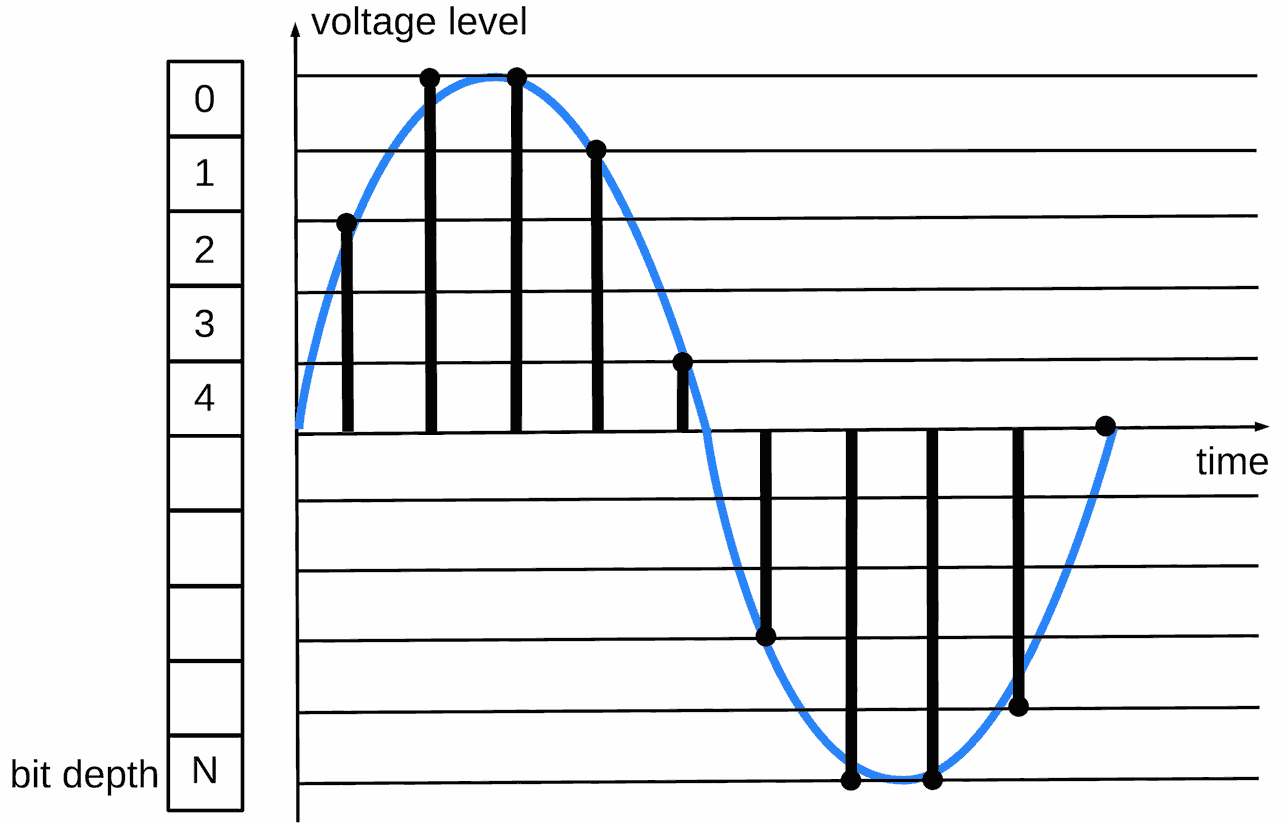
\includegraphics[scale=0.2]{./immagini/discretizazione-suono.png}
	\end{center}
	\caption{Conversione segnale audio analogico digitale}\label{fig:SR-bitdepth}
\end{figure}
Come possibile osservare nell'immagine di esempio \ref{fig:SR-bitdepth} l'input che riceve un ADC è un segnale analogico, un voltaggio identificato con il sinusoide colorato di blu, continuo e senza interruzioni. Questo voltaggio verrà registrato a intervalli regolari di tempo dal convertitore, andando ad approssimare il segnale rilevato al bit che più si avvicina ad esso, ad esempio vediamo he alla prima rilevazione l'ADC approssima il segnale analogico al secondo bit, dal momento che era il bit a cui il segnale si avvicinava maggiormente. Il secondo come il terzo vengono approssimati al bit 0, e così via fino a che non termina il segnale. Questi punti verranno poi interpolati tra loro dai programmi che permettono di effettuare le registrazioni e salvarli nei formati di preferenza, nel nostro caso ARFF o WAV.
I valori di SR e bit depth sono solitamente limitati dall'hardware, in questo caso la scheda audio.

\subsection{Formati WAV e AIFF}
Questi formati audio sono molto importanti, come detto all'inizio del capitolo, perché consentono di salvare tracce audio senza alterare le caratteristiche sonore e dinamiche dell'audio. Questo quantitativo di informazioni deve però essere pagato in termini di memoria, infatti i file salvati in questi formati possono arrivare ad essere di grandi dimensioni anche per registrazioni di pochi minuti. A questo proposito viene introdotto negli anni '90, con l'avvento dell'audio digitale, il formato mp3, che consente di effettuare un \emph{downsampling} dell'audio riducendo lo spazio di memoria necessario per l'archiviazione. Questa procedura di compressione delle informazioni, riduce però la qualità, non strettamente percepibile da rovinare l'ascolto, ma a sufficienza da rendere questo tipo di file inadatto ad analisi attente come missaggio, o mixing in inglese\footnote{Fase di miscelazione dei suoni in produzione audio} e mastering\footnote{Fase successiva al missaggio svolta su una singola traccia ottenuta dal missaggio per consentire la migliore riproduzione sonora dell'audio su diversi dispositivi} per gli studi di registrazione.

\section{Features utilizzate}
Visto come sono formati i file audio da utilizzare, WAV o AIFF, sono state scelte le seguenti features da utilizzare per l'approccio deciso di ML per descrivere un'onda sonora: la \emph{media}, la \emph{varianza}, la \emph{media della derivata prima} e  \emph{della derivata seconda}.

%CHE DEVE ESSERE TRATTATO NEL DISCRETO, VEDI FILE AUDIO: SOTTO PUNTI WAV E AIFF


%dell'algoritmo che hai usato J48 anche se già specificato in capitolo 1,  spiega poi passaggio da NOTA NON-NOTA (problema iniziale: vedere se possibile riconoscere nota da non nota) a 5 classi(riconoscere nota a vari livelli: 100\% ... 0\%). 
%
%VEDI APPUNTI PER CAPITOLO 2/3